% ======================================================================
\section{The final system}\label{sec:system}

This section describes the final system exactly as the code runs it: the configuration
\cfgv{config.use_shipped()} (\fp{config.py}), frozen on 2 Oct 2026 under git tag
\texttt{detector-frozen-2026-10-02}. Where the scoring harness and the live pipeline differ, the difference is
stated (Section~\ref{sec:parity}). Every value below gives its configuration variable;
Appendix~\ref{app:config} lists them all.

\subsection{Overview}
Figure~\ref{fig:pipeline} shows the data flow. In words, for one video:
\begin{enumerate}
  \item \textbf{Hear candidates.} Two sound detectors listen to the whole clip: BEATs (a 527-class tagger) and
        FlexSED (a detector that finds sounds by name). Anything they hear strongly enough, for at least 0.3\,s,
        becomes a candidate with a start and an end.
  \item \textbf{Check candidates.} A chain of vetoes removes candidates that only one model claims. Weak sounds
        that the detectors almost missed get second opinions from two audio-language ``listeners''
        (Qwen3-Omni and Audio Flamingo Next) and a third audio model (DASM).
  \item \textbf{Witness rule.} A remaining candidate needs a witness: DASM clearly hears it, or both listeners name
        it, or one listener names it \emph{and} the vision model finds the sound plausible in the scene.
  \item \textbf{On-screen check (the gate).} A vision--language model (Qwen3.8-27B) looks at the frames around each
        sound. If the thing making the sound is visibly making it, no picture is shown.
  \item \textbf{Clean the display.} Repeats close together become one picture; a listener decides whether two
        same-type pictures up to 8\,s apart are one continuing sound; a picture is dropped when its event is
        visibly happening.
  \item \textbf{Draw.} A short, guarded text prompt is written for each remaining sound; Qwen-Image draws it; a
        checker asks whether the picture shows the intended thing and redraws up to five times.
  \item \textbf{Compose.} The pictures are shown in up to three fixed slots beside the video, each while its sound
        plays (at least 1.5\,s).
\end{enumerate}

\begin{figure}[t]
\centering
\resizebox{\linewidth}{!}{%
\begin{tikzpicture}[
  node distance=4mm and 6mm,
  box/.style={draw, rounded corners=2pt, align=center, font=\scriptsize, minimum height=8mm, text width=2.5cm, fill=white},
  model/.style={font=\tiny\itshape, text=gray!70!black, align=center},
  arr/.style={-{Stealth[length=2mm]}, thick}]
\node[box, fill=gray!10] (in) {video (mp4)};
\node[box, right=of in] (s1) {1 audio\\16 kHz mono};
\node[box, below=of in] (s2) {2 frames\\objects (context)};
\node[box, below=of s1] (s3) {3 speech\\transcript (context)};
\node[box, right=of s1, text width=3.0cm, fill=blue!6] (s4a) {4a candidates\\BEATs $\cup$ FlexSED};
\node[box, below=of s4a, text width=3.0cm, fill=blue!6] (s4b) {4b vetoes, listener\\rescue, witness rule};
\node[box, below=of s4b, text width=3.0cm, fill=blue!6] (s4c) {4c onset refinement,\\rescue filters};
\node[box, right=of s4a, text width=2.9cm, fill=orange!8] (s5) {5 on-screen gate\\3 votes, every 5-s stretch};
\node[box, below=of s5, text width=2.9cm, fill=orange!8] (s5b) {5b kinship, subject\\(what to draw)};
\node[box, below=of s5b, text width=2.9cm, fill=green!7] (s6) {6 picture + check\\(up to 5 tries)};
\node[box, below=of s6, text width=2.9cm, fill=green!7] (s6b) {6b display: merge,\\group, depict-event};
\node[box, left=of s6b, text width=3.0cm, fill=gray!10] (out) {7 side-by-side video};
\draw[arr] (in) -- (s1);
\draw[arr] (in) -- (s2);
\draw[arr] (s1) -- (s3);
\draw[arr] (s1) -- (s4a);
\draw[arr] (s4a) -- (s4b);
\draw[arr] (s4b) -- (s4c);
\draw[arr] (s4a.east) -- (s5.west);
\draw[arr] (s4c.east) -- ++(3mm,0) |- (s5.west);
\draw[arr] (s5) -- (s5b);
\draw[arr] (s5b) -- (s6);
\draw[arr] (s6) -- (s6b);
\draw[arr] (s6b) -- (out);
\draw[arr, dashed, gray] (s2.south) |- ++(0,-4mm) -| (s5b.south west);
\draw[arr, dashed, gray] (s3.east) -- (s4b.west);
\node[model, below=0.5mm of s4c] {BEATs, FlexSED, PANNs, DASM,\\Qwen3-Omni, Audio Flamingo Next, FineLAP};
\node[model, above=0.5mm of s5] {Qwen3.8-27B};
\node[model, right=0.5mm of s6, text width=1.6cm] {Qwen-Image-2512 + Qwen3.8 + EasyOCR};
\node[model, right=0.5mm of s6b, text width=1.6cm] {Qwen3-Omni (group), Qwen3.8 (depict)};
\end{tikzpicture}}
\caption{The final pipeline. Blue: detection (stage 4); orange: the on-screen decision (stage 5); green: pictures and
display. Dashed: context only (objects and transcript never decide on their own). The scene check of the witness
rule in stage 4b also uses Qwen3.8-27B.}
\label{fig:pipeline}
\end{figure}

\begin{figure}[t]
\centering
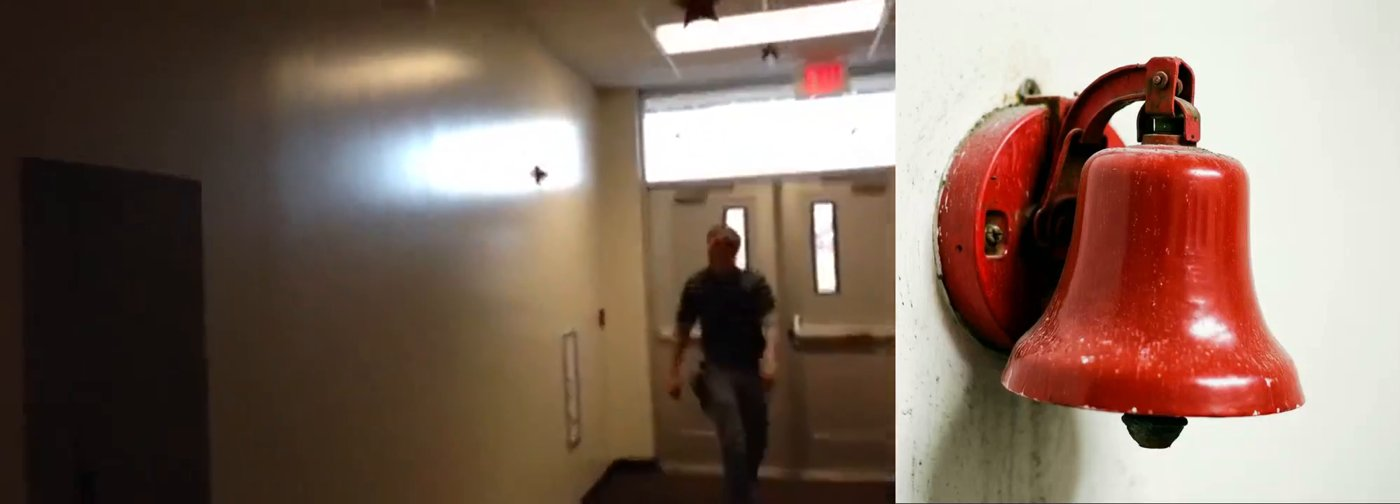
\includegraphics[width=\linewidth]{figures/example_fire_alarm.jpg}
\caption{Output of the final system on a development clip (AudioSet-Strong, a corridor). A fire alarm rings
from 9.0\,s; the alarm bell itself is not in the frame. The system detects \emph{Alarm}, the on-screen check finds no
visible source, and the panel on the right shows the generated picture from 8.9\,s while the alarm sounds. In the
scoring this is a hit.}
\label{fig:example}
\end{figure}

\subsection{Stages at a glance}
\begin{table}[h]
\centering\small
\caption{Stages, models and key parameters of the final system (in the order of \fp{src/pipeline.py}).}
\label{tab:stages}
\begin{tabular}{L{0.4cm}L{2.4cm}L{5.0cm}L{6.4cm}}
\toprule
\# & stage & model / tool & key parameters \\
\midrule
1 & audio & ffmpeg & mono WAV, 16 kHz (\cfgv{SAMPLE_RATE}) \\
2 & frames, objects & OWLv2 (\fp{owlv2-base-patch16-ensemble}) & 6 frames, threshold 0.20; context only, never silences a sound \\
3 & speech & faster-whisper \texttt{base}, int8 & transcript used only to ask whether people react to a sound; never drawn \\
4 & sound events & BEATs iter3+ AS2M; FlexSED; PANNs CNN14; DASM; Qwen3-Omni-30B-A3B; Audio Flamingo Next; FineLAP & 16 ordered steps, Table~\ref{tab:stage4} \\
5 & on-screen gate & \texttt{Qwen/Qwen3.8-27B}, greedy, thinking off & 6 frames per $\leq$5-s stretch, 3 votes, majority; silenced only if every stretch is visible \\
5b & subject & Qwen3.8-27B + word lists & 2--6 word phrase; speech text never used \\
6 & picture & \texttt{Qwen/Qwen-Image-2512} & 1024$^2$, 50 steps, true CFG 4.0; check-and-redraw $\leq$5 tries \\
6b & display & Qwen3-Omni (group), Qwen3.8 (depict) & merge gap 2.5\,s, min.\ 1.5\,s on screen, $\leq$1\,s past the end, group $\leq$8\,s, 3 slots \\
7 & composite & ffmpeg libx264 & 720-px panel, 25 fps \\
\bottomrule
\end{tabular}
\end{table}

\subsection{Stage 4: detection}\label{sec:stage4}
Stage 4 is where most of the development effort went. It turns the audio into a list of timed candidate sounds,
each with a family label and a confidence. The entry point is \cfgv{detect_events}
(\fp{src/stage4_audio_event_detection/__init__.py}); unions and vetoes are in \cfgv{fuse_flexsed}, the filters on
rescued spans in \cfgv{filter_rescued}.

\subsubsection{Models}
\begin{description}[style=nextline]
  \item[BEATs] iter3+ fine-tuned on AudioSet-2M (checkpoint
        \texttt{BEATs\_iter3\_plus\_AS2M\_finetuned\_on\_AS2M\_cpt2}). It scores a whole window, so it is run on 2-s
        windows every 0.25\,s; the first two seconds are mirror-padded so a sound at the very start can be heard; each
        window's score is stamped 0.5\,s before the window ends, so a detected start is never earlier than the true one.
  \item[FlexSED] an open-vocabulary, frame-level detector~\cite{hai2025flexsed}: a self-supervised audio encoder plus
        a CLAP text encoder (\texttt{laion/clap-htsat-unfused}), trained on AudioSet-Strong. It is asked one plain
        query per family over the 215 \emph{depictable} families (\fp{benchmark/gold/depictable_vocab.json}), 25 frames
        per second. It hears quiet sounds under speech and music far better than BEATs.
  \item[PANNs CNN14] (sound-event version, 32 kHz) used only as a clip-level veto.
  \item[DASM] Detect Any Sound Model (ACM MM 2025; weights \texttt{CPF2/detect\_any\_sound}), queried with ``sound of
        $\langle$family$\rangle$'' over the same 215 families, 50 frames per second. Used as a witness and a vote.
  \item[Listeners] \texttt{Qwen/Qwen3-Omni-30B-A3B-Instruct} and \texttt{nvidia/audio-flamingo-next-hf}. Each is asked
        a yes/no question (``Is the sound of $\langle$family$\rangle$ present in this recording?'', scored as the logit of
        \emph{yes} minus the logit of \emph{no}) and an open inventory (``List every distinct non-speech sound you hear in
        this recording, one per line, most prominent first.''). An inventory line names a family if it matches its name,
        an AudioSet synonym, a parent or a child, or else has sentence-embedding cosine $>0.6$
        (\texttt{all-mpnet-base-v2}). The audio cut is the candidate span $\pm 1$\,s, at least 1\,s long.
  \item[FineLAP] (\texttt{AndreasXi/FineLAP}, MIT) a frame-level audio--text model used as a last veto on rescued sounds.
\end{description}

\subsubsection{Steps in execution order}
Table~\ref{tab:stage4} gives the 16 steps. Two words are used throughout: a \emph{rescued} span is one added by a
listener after the detectors missed it; a \emph{twinned} span is one both detectors raised.

{\small
\begin{longtable}{L{0.4cm}L{2.8cm}L{7.9cm}L{3.2cm}}
\caption{Stage 4 of the final system, step by step.}\label{tab:stage4}\\
\toprule
\# & step & rule & variable(s) \\
\midrule\endfirsthead
\toprule \# & step & rule & variable(s) \\ \midrule\endhead
\bottomrule\endfoot
1 & BEATs spans & a span of any class where the window score $\geq 0.175$; kept if $\geq 0.3$\,s long; confidence = peak & \cfgv{AED_THRESHOLD} 0.175, \cfgv{AED_MIN_DUR} 0.3 \\
2 & FlexSED spans & same extractor on FlexSED frames at bar 0.8, $\geq 0.3$\,s & \cfgv{FLEXSED_BAR} 0.8 \\
3 & twin union & a FlexSED span with a same-family BEATs span within 1\,s is merged into it (earlier start kept; confidence = the stronger side, rescaled); otherwise kept as FlexSED-only & \cfgv{TWIN_MAX}, \cfgv{UNION_START} min \\
4 & mirror veto + listener keep & a BEATs-only span is dropped if FlexSED's top query in its window is another family $\geq 0.7$ while its own family is $<0.4$; put back if the Qwen listener accepts it and an inventory names it & \cfgv{MIRROR_VETO} 0.7, \cfgv{KEEP_NEEDS_V4} \\
5 & masked-weak veto & a BEATs-only span with confidence $<0.5$ under speech or music ($\geq 0.3$) is dropped unless a listener accepts it & \cfgv{MASKED_WEAK_VETO} \\
6 & DASM clip veto & a span whose family DASM never reaches 0.0839 anywhere in the clip is dropped unless a listener keeps it & \cfgv{DASM_CLIP_VETO} \\
7 & \textbf{witness rule} & pass if DASM $\geq 0.35$ for the family within the span $\pm 0.5$\,s; else pass if \emph{both} listener inventories name the family; if exactly one does, ask the scene check (Section~\ref{sec:scenecheck}); otherwise drop & \cfgv{DASM_LOCAL_VETO} 0.35, \cfgv{DASM_LOCAL_KEEP} both, \cfgv{SCENE_FIT_LOGIT} \\
8 & inventory keep & a span with confidence $\geq 0.35$ for which both inventories exist and neither names its family (or a descendant) is dropped, unless DASM $\geq 0.575$ within $\pm 0.5$\,s & \cfgv{KEEP_NEEDS_V4_ALL} onto, \ldots\cfgv{_DASM_KEEP} \\
9 & band-twin pull & the start moves back to an earlier same-family FlexSED run ($\geq 0.5$) that ends $\leq 1$\,s before and starts $\leq 1.5$\,s before it & \cfgv{BAND_TWIN_PULL} 0.5 \\
10 & continuation veto & a span is dropped when a same-family FlexSED run ($\geq 0.5$) began $\geq 1.5$\,s earlier and is still on at its start (it is a later piece of a sound already shown) & \cfgv{CONTINUATION_VETO} 0.5 \\
11 & FlexSED veto & a span whose family FlexSED never reaches 0.3 in the clip is dropped & \cfgv{FLEXSED_VETO} 0.3 \\
12 & PANNs veto & a FlexSED-only span whose family PANNs never reaches 0.05 is dropped unless a listener accepts it & \cfgv{PANNS_VETO} 0.05 \\
13 & listener band rescue & a FlexSED run with peak in $[0.5, 0.8)$ and no same-family span is added if accepted: peak $\geq 0.6$ needs the Qwen inventory; $<0.6$ needs both inventories & \cfgv{LISTENER_RESCUE}, \cfgv{LISTENER_RULE} TIER \\
14 & DASM rescue & a DASM run ($\geq 0.575$) with no detector span nearby is added if both inventories name the family and the family is new in the clip & \cfgv{DASM_RESCUE}, \ldots\cfgv{_NEW_ONLY} \\
15 & onset refinement & for BEATs spans: silence the first $t$ seconds of the first firing window for 26 values of $t$ and take the first $t$ at which 10\,\% of the class evidence is gone; never earlier than the detected start & \cfgv{ONSET_CAM}, \cfgv{ONSET_MONOTONE} \\
16 & rescued-span filters & on rescued spans only: FineLAP $\geq 0.329$; DASM $\geq 0.575$ within $\pm 0.5$\,s; at most one rescued span per family per clip (the earliest) & \cfgv{FINELAP_VETO} 0.329, \cfgv{LISTENER_DASM_VOTE}, \cfgv{LISTENER_ONCE} \\
\end{longtable}
}

The DASM thresholds 0.0839 and 0.575 and the FineLAP bar 0.329 were calibrated during development
(Appendix~\ref{app:history}); every other threshold was set once and not tuned on the test set. Steps 4--8 and 12--16 depend on listener answers that are computed from a first pass
with the September baseline (the candidate ``pools''), so the final detector cannot run without that pass
(Section~\ref{sec:repro}).

\subsubsection{The scene check}\label{sec:scenecheck}
When exactly one listener names a weak sound, the witness rule asks the vision model whether the sound is plausible
in the scene. The span is cut into stretches of about 5\,s; for each, six frames from 1\,s before to 1\,s after are
shown with the question ``Could the sound of $\langle$label$\rangle$ plausibly be heard in this scene? Answer yes or
no.'' and its negated twin. The answer is read from the first output token as
$d = m(Q) - m(\bar Q)$, where $m$ = max logit over \{yes, Yes\} minus max logit over \{no, No\}; $d>0$ counts as yes,
and the sound passes if most stretches say yes. Reading the logits replaced an earlier text answer that was cut
off after four tokens on 10--15\,\% of calls (Appendix~\ref{app:history}).

\subsection{What may be drawn}\label{sec:labelfilter}
The label filter (\cfgv{LABEL_FILTER = "depictable"}, \fp{src/labels.py}, \cfgv{is_salient_nonspeech}) maps every
label to its family and removes: speech with words and its descendants (Speech, Conversation, Narration, Hubbub,
Whispering, \ldots), music and singing and their descendants, the ``channel, environment and background'' branch,
silence and generic labels, textures (Breathing, Rumble, Hum, Whir, Rustle, Wind and its descendants), and labels
with no clear source (Sound effect, Onomatopoeia, generic impacts). Everything else is drawable, including non-word
vocal events (shout, scream, laughter, cough, snoring). FlexSED and DASM are asked only about the 215 drawable families.

\subsection{Stage 5: the on-screen gate}\label{sec:gate}
Stage 5 first groups the detections by family at the display bar 0.35 (\cfgv{DISPLAY_THRESHOLD}); firings of one
family less than 1\,s apart are one burst. It then asks Qwen3.8-27B, with greedy decoding and thinking off, for every
burst:

\begin{enumerate}
  \item The burst is cut into $k = \max(1, \operatorname{round}(\text{length}/5))$ stretches; each stretch gets
        six frames, evenly from 1\,s before to 1\,s after it.
  \item Three votes per stretch (prompts in Appendix~\ref{app:prompts}):
    \begin{description}
      \item[name] ``Name the thing in these frames that is making that sound \ldots{} or answer exactly: nothing.''
            A name that shares a word with the label counts yes; otherwise a text-only question asks whether that
            thing could make the sound.
      \item[a/b] ``(a) you can SEE $\langle$label$\rangle$ happening on screen -- the source is in the frames and
            visibly making that sound; (b) $\langle$label$\rangle$ is not visibly happening.'' Asked in both option
            orders; if the two answers disagree the vote abstains.
      \item[describe] a 25-word description of the frames; yes if it names the sound or the named thing, else the
            same text-only question.
    \end{description}
  \item A stretch is visible if yes-votes outnumber no-votes. The sound is silenced only if \emph{every} stretch is
        visible; otherwise its picture is kept for the whole burst.
  \item \textbf{Kinship.} A sound is also silenced if a silenced sound of the same source overlaps it in time
        (live: only when the visible label is the same or more specific; Section~\ref{sec:parity}).
  \item \textbf{Speech context.} If at least four words of speech fall within 3\,s of a sound, a text-only question
        asks whether the people react to it; a yes gives the sound priority for a slot and can rescue a sound just
        below the display bar. Speech never enters a picture.
  \item \textbf{Disambiguation.} Two different labels with starts and ends within 0.6\,s are one sound with two
        names; the frames are shown with ``which is it, (a) A or (b) B or (c) cannot tell?'' in both orders.
\end{enumerate}
The rule ``silence only if every stretch is visible'' leans toward showing: a sound whose source leaves the frame
for one stretch keeps its picture.

\subsection{Stage 5b and 6: what the picture shows}\label{sec:pictures}
\paragraph{Subject.} The picture prompt is built from the detector's label, not from free text. A resolve step asks
the VLM for at most two qualifier words plus the head word of the source (accepted only if it ends with the head
word, names no person and no forbidden kind), then a 3--6-word event phrase. Word-list guards remove persons, places
and makers from other ontology branches. Action labels are drawn as their maker (\emph{bark} $\to$ a barking dog)
from a hand table, ontology senses (\emph{Honk} = goose), or a closed VLM choice on the frames. Sounds that are best
shown as a word (\emph{Whoosh}, \emph{Thud}, \emph{Bang}, \emph{Smack}, \emph{Whack}) get a fixed comic burst card,
and a few sounds a fixed template (thunder = ``one large lightning bolt striking down from a dark storm cloud'').

\paragraph{Generation.} The prompt is the subject plus a fixed tail (``the whole thing fully in frame, caught at the
moment it makes the sound with its visible effect, one large subject filling the picture, plain white background'')
and a negative prompt (scenery, landscape, room interior, street, buildings, text, letters, watermark). Qwen-Image-2512
draws it at 1024$\times$1024 with 50 steps and true CFG 4.0; the seed is a hash of clip, label and start time, so a
run is repeatable.

\paragraph{Check and redraw.} The same Qwen3.8-27B is shown the picture with a shuffled multiple-choice question
(the intended thing, known look-alikes, generic confusions such as ``a person'' or ``a building'', ``something
else''); EasyOCR rejects a picture that contains a readable word. A failed picture is redrawn with a new seed and the
confusing thing added to the negative prompt, up to five tries; if all fail, a word card with the sound's name is
shown. The check was validated on known cases (7 of 7 known-bad pictures caught, 33 of 33 deliberately wrong ones
refused, 3 of 68 good ones refused, 113 of 115 answers unchanged on reshuffling) but never calibrated against a human
rater (Section~\ref{sec:disclosures}).

\subsection{Stage 6b: display}\label{sec:display}
\begin{enumerate}
  \item \textbf{Depict-event}: a picture is dropped if, on six frames around its start, the VLM says its
        event is visibly happening (and its negated twin agrees) \emph{and} a maker the gate named could be mistaken
        for the sound.
  \item \textbf{Repeat merge}: bursts of one label join into one appearance if the gap from the previous real end is
        $\leq 2.5$\,s (\cfgv{MERGE_GAP}).
  \item \textbf{Dwell}: each appearance stays at least 1.5\,s (\cfgv{MIN_DWELL}) and at most 1\,s past the real end
        of the sound (\cfgv{MAX_AFTER_END}).
  \item \textbf{Grouping}: for two same-family pictures whose gap is at most 8\,s, Qwen3-Omni hears the
        audio from just before the first ends to just after the second starts and is asked whether the second is ``the
        same continuing sound \ldots{} (one alarm or engine with a short pause)'' or ``a new, separate event
        (\ldots{} a second bark, knock or shot)''; both option orders must say ``same'' to merge.
  \item \textbf{Slots}: at most three pictures at once, each in a fixed slot; if more overlap, sounds people react to
        come first, then confidence. A slot is empty when its sound is silent.
\end{enumerate}

\subsection{Scored harness versus live pipeline}\label{sec:parity}
The numbers in this report come from the scoring harness, which runs the pipeline's own stage-4 functions on cached
model scores and replays the gate answers of a full run. A parity check (\fp{benchmark/gold/parity_check.py}) and an
independent re-export of every decision (the Decision Inspector, Section~\ref{sec:repro}) reproduce the published
counts exactly (0 of 159 clips differ). The live configuration \cfgv{use_shipped()} differs from the scored one in
four known ways:
\begin{itemize}
  \item \textbf{Kinship direction.} Live: a visible label silences only the same or a more specific label. Scored:
        either direction. This was a deliberate logic fix made after the scored tables; its effect on the final
        numbers was not re-measured.
  \item \textbf{Picture end.} Live pictures end at most 1\,s after their sound; scored pictures had no cap. Starts --
        the scored quantity -- are identical; on 3 TEST clips a picture ends 0.04--0.38\,s earlier live.
  \item \textbf{Subject path.} The scored runs used the older depiction path, which can drop a sound whose depiction
        fails twice and feeds a similarity-based merge; the live path never drops a sound at this step. No end-to-end
        equality test of \fp{main.py} against the scored numbers exists.
  \item \textbf{Pictures.} Scored runs used placeholder or FLUX.1-schnell pictures; the live system uses Qwen-Image
        with the check. Pictures are not part of the per-sound score.
\end{itemize}
